\begin{exercise}{Système thermomécanique}{2}{Sup, spé}
{Thermodynamique}{lelay}

On considère un système thermomécanique définit comme suit : Dans un conduit vide de section $S$ et de longueur $\ell_0$, on place une paroi reliée à une extrémité du conduit par un ressort de raideur $k$ et de longueur à vide $\ell_0$. Entre l'autre extrémité et la paroi, on place une certaine quantité d'un gaz du indice adiabatique $\gamma$.

\begin{center}
    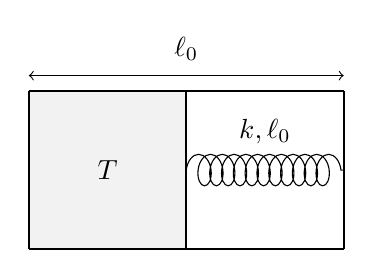
\begin{tikzpicture}
    \draw[<->] (0,1.2) -- (4, 1.2);
    \draw (2,1.2) node[above=2pt] {$\ell_0$};
    
    \fill[black!5]  (0,-1) rectangle (2,1);
    \draw[thick] (0,-1) -- (0, 1);
    \draw[thick] (0,-1) -- (4,-1);
    \draw[thick] (0, 1) -- (4, 1);
    \draw[thick] (2,-1) -- (2, 1);
    \draw (1,0) node[anchor=center] {$T$};
    
    \draw[decoration={aspect=0.6, segment length=1.5mm, amplitude=2mm,coil},decorate] (2,0) -- (4,0);
    \draw[thick] (4,-1) -- (4, 1);
    \draw (3,0) node[above=6pt] {$k, \ell_0$};
    
    \end{tikzpicture}
\end{center}

\begin{questions}
    \questioncours Capacités thermiques et coefficient isentropique.
    \question Initialement, le gaz est à la température $T$. Exprimer l'énergie potentielle du ressort en fonction de $T$.
    \question On fournit une certaine quantité de chaleur $Q$ au système. Que se passe-t-il ? 
    \question Donner la définition et exprimer ${C_{V}}_{m}$ la capacité thermique isochore molaire du système étudié.
\end{questions}

\end{exercise}

\begin{solution}

\begin{questions}
    \questioncours $c_p = c_v + nR$
    \question Si on note $x$ le déplacement du ressortr, alors $V = x S$, $P = kx/S$ hence $E_p = \frac12 kx^2 =\frac12 PV$. Or $PV =nRT$ d'où $E_p = nRT/2$
    \question Ca bouge. Bilan d'énergie : $Q = \Delta U_\text{gaz} + \Delta E_p = c_v \Delta T + nR/2\Delta T$
    \question  ${C_{V}}_{m} = \Delta U_\text{tot}/\Delta T = c_v + nR/2$
\end{questions}

\end{solution}